\section{法兰盘图样}\label{sec:falan}

{\bfseries 知识目标}
\begin{itemize}
\item 掌握layer命令和图层定义和使用方法
\item 掌握xline命令的使用方法
\item 掌握circle命令的使用方法
\item 掌握多边形命令的使用方法
\item 掌握图形阵列命令的使用方法
\item 掌握trim编辑命令的使用方法
\end{itemize}

{\bfseries 技能目标}
\begin{itemize}
\item 能够完成简单图样的绘制
\item 具备用AutoCAD图层管理图线的能力
\end{itemize}

\noindent
\begin{figure}[htbp]
\centering
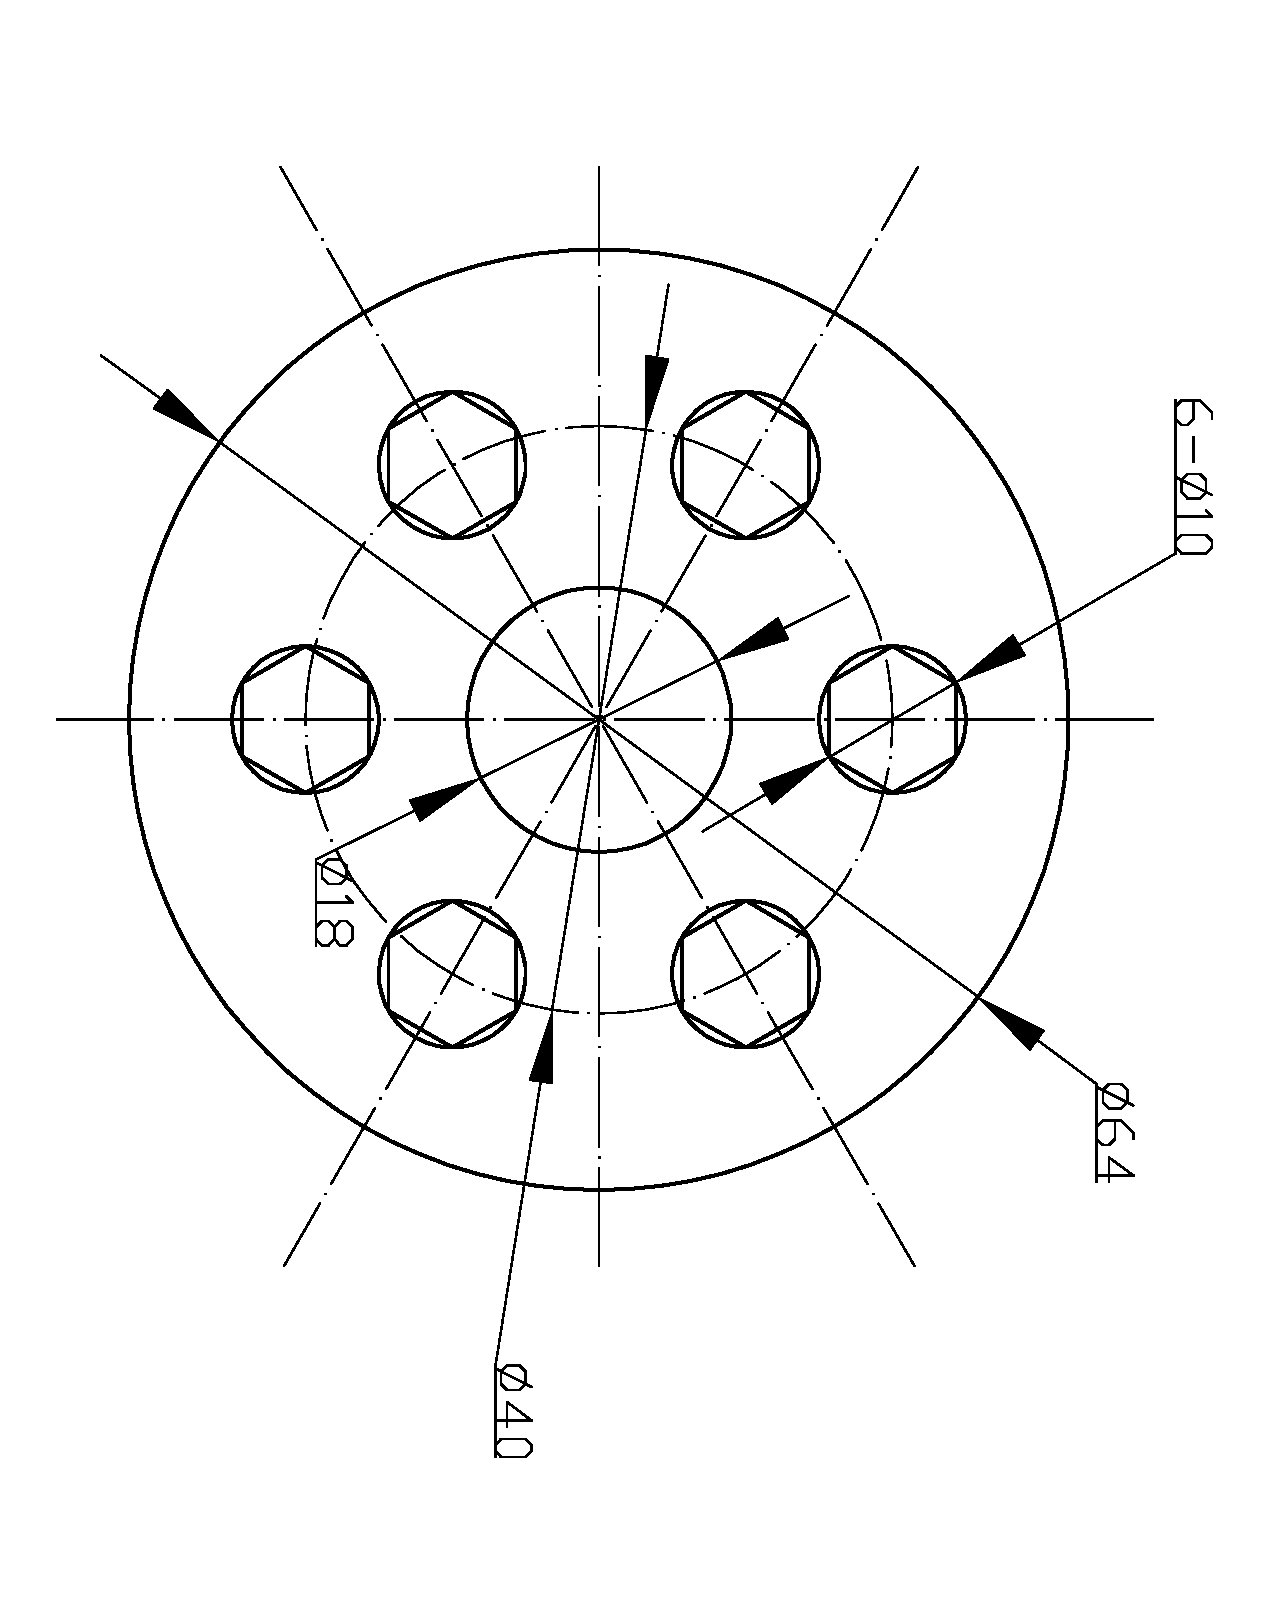
\includegraphics[scale=0.45,angle=90]{shu2.pdf}
\caption{法兰盘图样}\label{fig:renwu2}
\end{figure}

\indent
本任务以完成\ref{fig:renwu2}所示法兰盘图形为目标,旨在让读者掌握用AutoCAD的图层来管理各种图线,并学会构造线、圆、多边形和图形阵列编辑命令的使用技巧。并让读者认识和理解图样抄画的步骤和顺序,形成图样绘制的基本职业习惯。

\subsection{图层设置与管理}
图\ref{fig:renwu2}所示的法兰盘图形一共包含了两种图线,一种是实线,一种是中心线。为了便于对不同类型的图线对象进行管理,我们需要应用AutoCAD的图层管理器来实现。所谓图层就是将属性相同的对象绘制在一张类似于透明的纸上,将不同属性的对象绘制在不同的透明的纸上,以便实现图形对象的分类管理,最后将所有的透明的纸叠加在一起就构成了整个图形。要实现图\ref{fig:renwu2}所示图形中实线和中心线两种图形对象的分层管理,需要用到AutoCAD中的layer命令来进行图层设置。

在命令行中输入Layer命令以执行【图层特性管理器】对话框,如图\ref{fig:tuchenguanliqi}所示。

\begin{figure}[htbp]
\centering
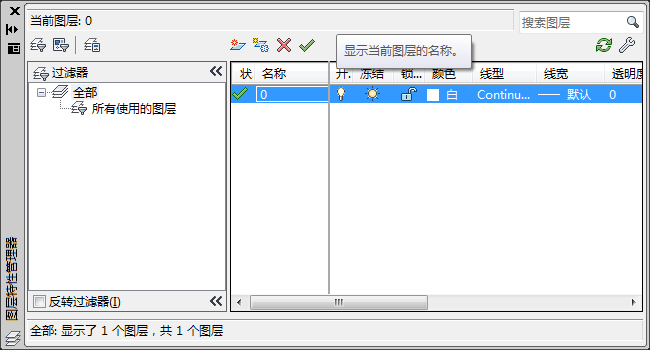
\includegraphics[scale=0.5]{Autocad_layer.png}
\caption{【图层特性管理器】对话框}\label{fig:tuchenguanliqi}
\end{figure}

单击新建图层按钮
\includegraphics[scale=0.5]{xinjiantuchen.png},新建一个实线图层和一个中心线图层。如图\ref{fig:xinjiantuchen}所示。
\begin{figure}[htbp]
\centering
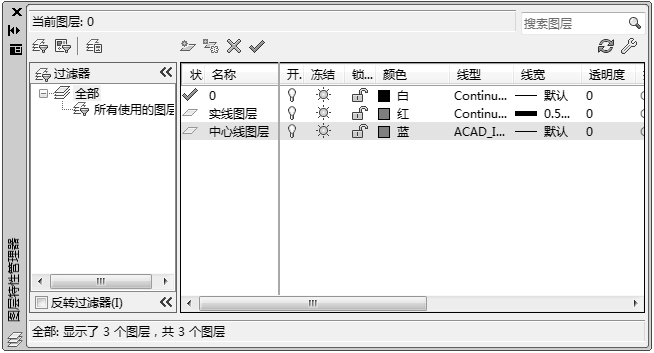
\includegraphics[scale=0.5]{xinjiantuchen1.png}
\caption{【新建图层】}\label{fig:xinjiantuchen}
\end{figure}

为了区别各个图层的对象,通常需要设置各个图层的颜色。此例中将实线图层的颜色设置为红色,将中心线图层设置为蓝色。具体设置方法是:单击要改变颜色的图层的颜色图标(即颜色框+颜色名),会弹出如图\ref{fig:colorset}所示的【选择颜色】对话框,选择想要的颜色即可完成设置。

\begin{figure}[htbp]
\centering
\begin{floatrow}
\ffigbox{\caption{【选择颜色】对话框}\label{fig:colorset}}{
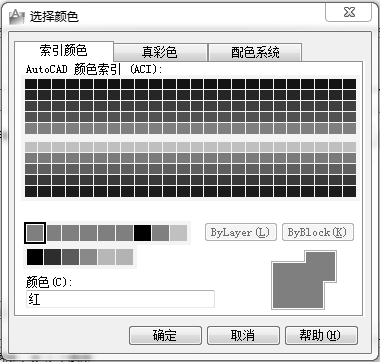
\includegraphics[scale=0.5]{colorset.png}
}
\ffigbox{\caption{【线宽】对话框}\label{fig:xiankuanset}}{
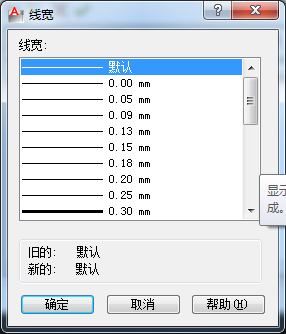
\includegraphics[scale=0.5]{linewidthset.png}
}
\end{floatrow}
\end{figure}
现在设置实线层的线宽,单击实线层中的线宽图标,弹出如图\ref{fig:xiankuanset}所示的【线宽】对话框,选择0.5mm的线宽作为实线层的线宽,单击确定即可。

接下来,按照规定将中心线图层的线型设置为ACAD\_ ISO04W100图线。具体设置方法为:单击中心线图层中的线型名,弹出如图\ref{fig:selectlinetype}所示的【选择线型】对话框。此时还没我所需要的线型,需要单击对话框中的【加载】按钮,弹出如图\ref{fig:linetypeload}所示的【加载或重载线型】对话框,选择ACAD\_ ISO04W100图线,并确定,以完成线型加载。最后在【选择线型】对话框中选中新加载的ACAD\_ ISO04W100图线,再一次单击确定,完成线型的设置。
\begin{figure}[htbp]
\centering
\begin{floatrow}
\ffigbox{\caption{【选择线型】对话框}\label{fig:selectlinetype}}{
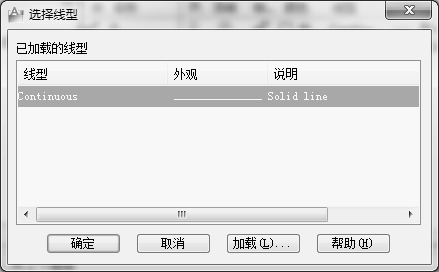
\includegraphics[scale=0.5]{AutoCAD_linetype.png}
}
\ffigbox{\caption{【加载或重载线型】对话框}\label{fig:linetypeload}}{
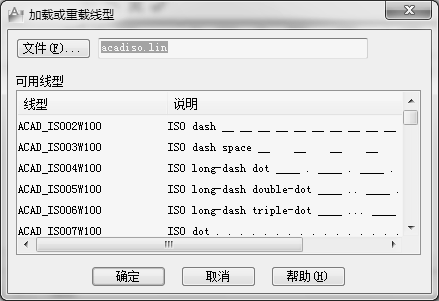
\includegraphics[scale=0.5]{linetype_load.png}
}
\end{floatrow}
\end{figure}

通过以上几个步骤,法兰盘的相关线型和图层就已经定义好了,可以开始绘制图形了。但在开始之前,我们需要先将中心线图层设置为当前图层。设置方法是:在【图层特性管理器】中选择中心线图层,再单击
\includegraphics[scale=0.6]{setlayercurrent.png}图标,即可将中心线层置为当前层。
\subsection{绘制图样}
\subsubsection{绘制中心线}
法兰盘图形的绘制要点关键在于中心线的绘制,因此首先需要绘制中心线,以便于定位。我们先用xline 命令绘制形的中心线,在命令行中输入xline并回车。

\begin{lstlisting}
%命令: XLINE 指定点或 [水平(H)/垂直(V)/角度(A)/二等分(B)/偏移(O)]: 32,32%
%指定通过点: $@1<0$%
%指定通过点: $@1<30$%
%指定通过点: $@1<90$%
%指定通过点: $@1<150$%
%指定通过点:%
\end{lstlisting}

接下来在命令行中输入circle命令来绘制中心线圆。

\begin{lstlisting}
%命令: CIRCLE %
%指定圆的圆心或 [三点(3P)/两点(2P)/切点、切点、半径(T)]: %
%int 于(用鼠标点击中心线的交点)%
%指定圆的半径或 [直径(D)]: 20%
\end{lstlisting}

通过完成上述操作便完成中心线的绘制。细心的读者可能已经发现了,这次所绘制的线并不仅仅只有一毫米长,而是无限长。用xline绘制的线称为构造线,通常用于绘制辅助线或者参考线。下面我们对xline和circle命令中的其它选项进行解释:

xline命令中【水平(H)】表示沿一点的水平方向创建一条构造线;【垂直(V)】表示沿一点的垂直方向创建一条构造线;【角度(A)】过一点并按一定角度创建一条构造线;【二等分(B)】表示行等分两条相交直线的夹角来创建一条构造线;【偏移(O)】表示创建与已知直线平行且距有指定距离的构造线。

circle命令中【三点(3P)】表示通过指定三个点来创建一个圆;【两点(2P)】表示通过指定直径上两端点来创建一个圆;【切点、切点、半径(T)】表示通过指定两个切点和半径来创建一个圆;在绘制圆的过程中,如果指定了圆心后会出现【直径(D)】选项,若输入D则会提示输入直径。另外如果所需要绘制与三个对象相切的圆则必须从【绘图】菜单【圆】子菜单中选择【相切、相切、相切(A)】项才能够实现。
\subsubsection{绘制实线}
完成法兰盘图形中心线的绘制后,我们就可以绘制其实线部分,由于当前的图层为中心线层,所以需要先切换当前图层为实现图层。切换当前图层的一种方法点击工具栏中的图层控制工具
\includegraphics[scale=0.6]{layercontrol.png},并在弹出的列表中选择实线图层。完成该操作后即将当前图层设置为实线图层。接下来,让我们开始绘制实线部分的图形:

\begin{lstlisting}
%命令: CIRCLE%
%指定圆的圆心或 [三点(3P)/两点(2P)/切点、切点、半径(T)]:%
% int 于(用鼠标点击中心线的交点)%
%指定圆的半径或 [直径(D)]: 9%
%命令:  CIRCLE %
%指定圆的圆心或 [三点(3P)/两点(2P)/切点、切点、半径(T)]:%
% int 于(用鼠标点击中心线的交点)%
%指定圆的半径或 [直径(D)]$ <9.0000>$: 32%
%命令: polygon %
%输入侧面数 $<4>$: 6%
%指定正多边形的中心点或 [边(E)]: int 于(用鼠标点击中心线的交点)%
%输入选项 [内接于圆(I)/外切于圆(C)]$ <$I$>$: c%
%指定圆的半径: 5%
%命令: circle %
%指定圆的圆心或 [三点(3P)/两点(2P)/切点、切点、半径(T)]:%
% int 于(用鼠标点击中心线的交点)%
%指定圆的半径或 [直径(D)]$ <32.0000>$: 5%
%命令:ARRAY%
%选择对象: 找到 1 个(选定要阵列的圆)%
%选择对象: 找到 1 个,总计 2 个(选定要阵列的六边形)%
%选择对象:  输入阵列类型 [矩形(R)/路径(PA)/极轴(PO)]$ <$极轴$>$:%
%类型 = 极轴  关联 = 是%
%指定阵列的中心点或 [基点(B)/旋转轴(A)]: int 于%
%输入项目数或 [项目间角度(A)/表达式(E)]$ <4>$: 6%
%指定填充角度(+=逆时针、-=顺时针)或 [表达式(EX)] $<360>$:%
%按 Enter 键接受或 [关联(AS)/基点(B)/项目(I)/项目间角度(A)/填充角度%
%(F)/行(ROW)/层(L)/旋转项目(ROT)/退出(X)] $<$退出$>$:%
\end{lstlisting}

在上述绘图过程中,我们用到了两个新命令polygon和array。

polygon命令用于绘制多边形,其中选项【边(E)】表示通过指定第一条边的端点来创建多边形;【内接于圆(I)】表示指定外接圆的半径,多边形的所有点位于外接圆上。;【外切于圆(C)】表示指定从正多边形圆心到各边中点的距离。

ARRAY命令用于创建在二维或三维图案中排列的对象副本,其中选项【矩形(R)】表示将对象副本分布到行、列和标高的任意组合;【路径(PA)】沿路径或部分路径均匀分布对象副本;【极轴(PA)】围绕中心点或旋转轴在环形阵列中均匀分布对象副本。

\subsubsection{完善图形}
经过上述操作,我们已经完成了法兰盘图样的绘制,但是由于我们在绘制中心线时使用的是xline,其中心线的长度是无限的,为了获得符合国家规定的中心线长度,我们需要对现在的中心线进行修改。修改教程是先画一辅助圆,再将辅助圆以外的修剪掉,最后将辅助圆删除即可。

\begin{lstlisting}
%命令:CIRCLE %
%指定圆的圆心或 [三点(3P)/两点(2P)/切点、切点、半径(T)]:%
%指定圆的半径或 [直径(D)]$<32.0000>$ :35%
%命令: trim%
%当前设置:投影=UCS,边=无%
%选择剪切边...%
%选择对象或 $<$全部选择$>$:  找到 1 个(选择圆)%
%选择对象:%
%选择要修剪的对象,或按住 Shift 键选择要延伸的对象,或%
%[栏选(F)/窗交(C)/投影(P)/边(E)/删除(R)/放弃(U)]:%
%选择要修剪的对象,或按住 Shift 键选择要延伸的对象,或%
%[栏选(F)/窗交(C)/投影(P)/边(E)/删除(R)/放弃(U)]:%
%选择要修剪的对象,或按住 Shift 键选择要延伸的对象,或%
%[栏选(F)/窗交(C)/投影(P)/边(E)/删除(R)/放弃(U)]:%
%选择要修剪的对象,或按住 Shift 键选择要延伸的对象,或%
%[栏选(F)/窗交(C)/投影(P)/边(E)/删除(R)/放弃(U)]:%
%选择要修剪的对象,或按住 Shift 键选择要延伸的对象,或%
%[栏选(F)/窗交(C)/投影(P)/边(E)/删除(R)/放弃(U)]: %
%选择要修剪的对象,或按住 Shift 键选择要延伸的对象,或%
%[栏选(F)/窗交(C)/投影(P)/边(E)/删除(R)/放弃(U)]:%
%选择要修剪的对象,或按住 Shift 键选择要延伸的对象,或%
%[栏选(F)/窗交(C)/投影(P)/边(E)/删除(R)/放弃(U)]:%
%选择要修剪的对象,或按住 Shift 键选择要延伸的对象,或%
%[栏选(F)/窗交(C)/投影(P)/边(E)/删除(R)/放弃(U)]:%
%选择要修剪的对象,或按住 Shift 键选择要延伸的对象,或%
%[栏选(F)/窗交(C)/投影(P)/边(E)/删除(R)/放弃(U)]:%
%命令: erase%
%选择对象: 找到 1 个%
%选择对象:%
\end{lstlisting}
\indent
经过上述修改后法兰盘图样就已经绘制完成了,并且符合国家标准的中心线长度要求。
\zhishi{图样绘制方法和步骤}
\subsection{CAD绘图流程}
\begin{enumerate}
\item 设置绘图界限。根据所绘图形的所需要采用了图幅大小设置AutoCAD的绘图区域界限。
\item 设置图层。根据绘图样所需要的线型创建图层并设置其颜色、线型、线宽等参数。
\item 画图框及标题栏(前两个任务省略了此过程)。
\item 确定绘图比例,布置图形,使图形在图纸上的位置和大小适中,各图形间应留有适当空隙及标注尺寸的位置。
\item 绘制图样。先画图形的基准线、对称线、中心线及有关定位尺寸线,再根据定型尺寸画主要轮廓线,然后由大到小,由整体到局部,画出其他所有图线。
\item 标注尺寸(将在后续任务中详细讲解)。
\end{enumerate}
\subsection{手工绘图流程}
\begin{enumerate}
\item 画图前的准备工作
    \begin{enumerate}
    \item 阅读必要的参考资料,对所画图形的内容与要求进行了解。
    \item 准备好必要的制图工具,将铅笔与圆规内的铅削好。
    \item 固定图纸
    \end{enumerate}
\item 画底稿
\begin{enumerate}
\item 画图框及标题栏(前两个任务省略了此过程)。
\item 确定绘图比例,布置图形,使图形在图纸上的位置和大小适中,各图形间应留有适当空隙及标注尺寸的位置。
\item 绘制图样。先画图形的基准线、对称线、中心线及有关定位尺寸线,再根据定型尺寸画主要轮廓线,然后由大到小,由整体到局部,画出其他所有图线。
\item 标注尺寸(将在后续任务中详细讲解)。
\end{enumerate}
\item 加深图线。按照先细后粗,先曲线后直线,先图形后尺寸,先图线后符号、文字的顺序,从上到下,从左到右进行。

\end{enumerate}
\clearpage
\endinput